\begin{figure*}[th!]
\centering
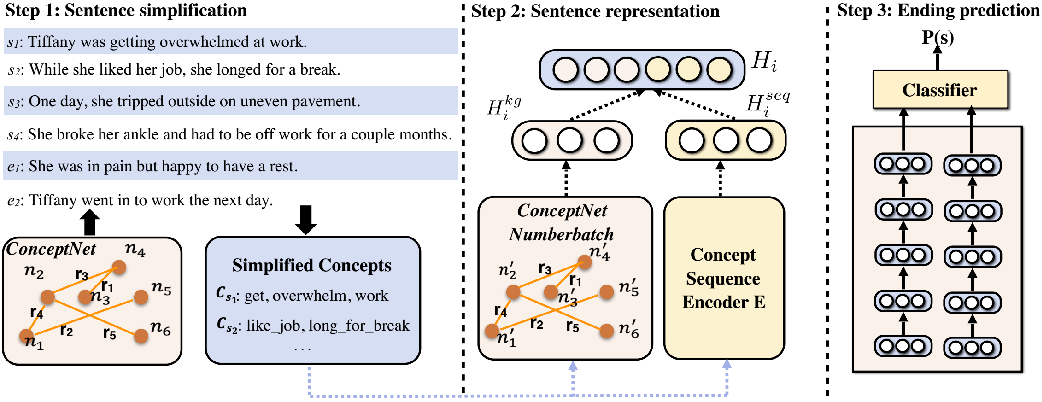
\includegraphics[width=2\columnwidth]{pictures/model}
\caption{Framework overview: our framework can be divided into three steps: 
sentence simplification, sentence representation and ending prediction. 
${n_1,...n_6}$ are the examples of token nodes in ConceptNet, 
${r_1,...r_6}$  are the commonsense relations between the nodes. 
${n_1^{'},...n_6^{'}}$ are the corresponding vector from Numberbatch\protect\footnotemark 
 which are trained on ConceptNet.
%\eve{what is 'main tokens'? need further explanation?}
% \KZ{Fix this figure. ``word sequence encoder''.}
}
\label{fig:model}
\end{figure*}
\footnotetext{\url{https://github.com/commonsense/conceptnet-numberbatch}}

\section{Approach}
\label{sec:approach}

%the approach part mainly contains 3 parts: simplification, skip-thought language model and commonsense reasoning embedding



Given the story context $\textbf{s} = (s_1, s_2, ..., s_L)$ of $L$ sentences,
the goal of the problem is to predict the correct ending from 
two candidate ending sentences $e_1$ and $e_2$.
We propose to refine and extend story sentence representations
by incorporating commonsense knowledge from ConceptNet for story ending prediction.
The architecture is shown in \figref{fig:model}, which consists of 
the following three steps. 
%We will introduce each step in the following subsections.
%First, we simplify each story sentence into a shorter sequence of words that
%only contains the key concepts in the sentence.
%Second, we construct the sentence representation from two aspects:
%the word sequence encoding of the simplified sentence,
%and encoding of the concepts in the context of a commonsense
%knowledge graph.
% Second, we represent the tokens in a sentence in two aspects.
% One aspect is  an unsupervised language model. The encoder hidden state can be seen as the text sentence vector. The other aspect is the structured commonsense knowledge from ConceptNet. We take in the token representation form Numberbatch, which contains token embeddings pretrained on ConceptNet. Combining the representation of these two aspects, we obtain a better commonsense representation of a story sentences.
%Finally, we train a GRU-based classification model that predicts the ending.

\subsection{Sentence Simplification}
\label{sec:sentence simplification}
% Just as the story example in \figref{fig:story} , we can find some words in a sentence is  important for story understanding and story reasoning. In the five-sentence stories (context with right ending and context with wrong ending), \textit{getting overwhelmed at work} $\rightarrow$ \textit{liked job longed for break} $\rightarrow$\textit{One day tripped outside uneven pavement} $\rightarrow$ \textit{broke ankle off work for a couple months}$\rightarrow$\textit{pain happy rest} construct a coherent story in semantic level, and obviously, this knowledge chain is more reasonable than \textit{getting overwhelmed at work} $\rightarrow$ \textit{liked job longed for break} $\rightarrow$\textit{One day tripped outside uneven pavement} $\rightarrow$ \textit{broke ankle off work for a couple months}$\rightarrow$\textit{went in to work next day}. Although the sentences are not complete, we can still refer to the right ending of the story.


%Our goal is to extract a sequence of of words 
%from an input sentence $s = \{w_1, ..., w_N\}$ 
%, namely $s'$, that accomodates only
%the key concepts and events in $s$ and 
%nothing else.~\footnote{The input sentences are 
%tokenized and lemmatized using Stanford CoreNLP~\cite{manning2014stanford} 
%in this work.}
%Because $s'$ is typically shorter than $s$, we say $s'$ is simplified
%from $s$.
Our goal is to extract a sequence of concepts $C_s$
from an input sentence $s = \{w_1, ..., w_N\}$ with N words. 
$C_s$ contains only the key concepts and events in $s$ and 
nothing else.~\footnote{The input sentences are 
tokenized and lemmatized using Stanford CoreNLP~\cite{manning2014stanford} }
We choose to use ConceptNet~\cite{speer2017conceptnet} as the source of
these concepts and events because of its comprehensive coverage of 
commonsense knowledge. Its exact coverage will be assessed 
in next section. 

The concepts and events in ConceptNet are
expressed in terms of short phrases, commonly made up of one or two words
such as ``break ankle''. While these phrases are meaningful and
understandable to human beings, they may not find exact match
in the input sentences, simply because people don't say ``break ankle'' in
normal text but instead ``break her ankle''.  
To remedy this problem, we develop a fuzzy match heuristics, that allows
$\lambda$ additional words to be inserted to a concept from ConceptNet
before exact matching in the input sentence.
% Typically, $\lambda$ ranges from 0 to 3.  
%We call $\lambda$ a ``simplification factor'' because 
%the larger the $\lambda$, the more concepts will be discovered from 
%the sentence and consequently the simplified sentence will be longer
%and ``not so simple.'' 
%On the other hand, larger $\lambda$ can also bring noise in the 
%simplified sentence since more extracted concepts will be incorrect. 
%We will evaluated the effect of $\lambda$ in \secref{sec:result}.

Another technical issue is that extracted concepts may overlap with 
each other in the input sentence. For example, from the sentence 
``She hope it would come back for more later'', we can extract the following
concepts: ``hope'', ``\textbf{come back}'', ``\textbf{come for}'', 
and ``more''. ``Come back'' and ``come for'' are both meaningful, and we keep 
them in $C_s$.
Afterwards, we remove duplicate concepts from $C_s$,
if it's contained by other concepts in the sequence. 
For example, we match ``come'' and ``come back'' in sentence. 
``Come'' will be deleted because it is the sub-sequence of the words in ``come back''. 
%\eve{'sub-sequence' is easier to understand than 'contained' for me. This is an 'overlap' but not 'contained' example.}
%Note that we keep concepts in original positions order in the sentence. 
The complete simplification
algorithm is shown in \algoref{alg:simplify}. $|c|$ means the number of words
of a concept $c$.

%The corresponding simplified output is a concept sequence $C_s = \{c_{s+1},..., c_{s+M}\}$
%representing $M$ mapped concepts within original sentence $s$.
%The simplification process with longest and 
%fuzzy match method is described in \algoref{alg:simplify}.  
%As a preprocessing step, we tokenize and lemmatize sentences with
%NLTK~\cite{loper2002nltk} and Standford CoreNLP~\cite{manning2014stanford}.

%For each concepts in ConceptNet $C$, If there exists a concept 
%$c_k = \{w_{k+1},...,w_{k+|c_k|}\}$ 
%denoting the k-th concept with $|c_k|$ words,
%which satisfies that $c_k$ is the subsequence of sentence $s$,
%then $c_k$ is extracted and appended to $C_s$. 
%If we use exactly consecutive sequence algorithm for matching, we will
% omit a lot of information, resulting in sparse data.
%For supporting a flexible matching, we introduce extra interval $\lambda$ which means 
%we allow a discontinuity in the spacing of $\lambda$ words. 
%For example, the concept ``broke ankle'' can be extracted
%from the sentence ``broke her ankle''. $\lambda$ here is equal to 1.
%Afterwards, we remove duplicated concepts from $C_s$,
%if it's strictly overlapped by other concepts in the sequence.
%Finally, all kept concepts are sorted by their original positions
%in the sentence.


% In order to choose the most important information from the sentence, we use ConceptNet token set  as a dictionary. Because it provides a large semantic graph which contains 1,500,000 nodes (concepts) and millions of edges for English. Its knowledge is collected from many sources that include expert-created resources, crowd-sourcing, and games with a purpose. We assume the tokens that appear in ConceptNet are important for commonsense understanding and reasoning.

% We use longest and fuzzy match for each sentence with the ~\algoref{alg:simplify}. We construct a dictionary which grouped by the first word of concepts. The keys are the first words. The values for each key are the concepts starting with the same dictionary key word. For the preliminary work, we tokenize and lemmatize sentence with NLTK and Standford’s CoreNLP tools ~\cite{manning2014stanford}. When traversing every word in a sentence, we choose the longest token. We also allow a discontinuous placeholder for fuzzy match. For example,  ``break'' in sentence ``She broke her ankle and had to be off work for a couple months''  should not be exactly matched with ``break ankle''  from dictionary. With the placeholder, we search extra one  continuous word in the sentence and will find this token belongs to the sentence. We can extract  ``broke ankle'' and  ``for couple months'' for this sentence. With this matching method, we can simplify a sentence $s_i$ in story $\textbf{s}$ to a token set. Let $c_{s_i} = c_{s_i}^{1},...,c_{s_i}^{D}$ be the $i_{th}$ sentence in all the serialized story sequence, where $D$ is the number of tokens matched in ConceptNet.

%\KZ{Redo this algo}
\begin{algorithm}[tb]
\small
\caption{Simplification algorithm}
\label{alg:simplify}
\textbf{Input}: ConceptNet $C$, sentence $s=\{w_1, ..., w_N\}$\\
\textbf{Output}: Concept sequence $C_s$ 
\begin{algorithmic}[1] %[1] enables line numbers
  % \Procedure{Simplify}{$C, S$}
  %   \STATE{$D$ \gets $xxx$}
  %   \FOR {Concept $c$ in $C$}
  %     \STATE{xxx}
  %   \ENDFOR
  % \EndProcedure
% \STATE Construct a dictionary $D$
% \FOR{token $x$ in ConceptNet nodes}
% \STATE $D[x.headword]$.append$(x)$
% \ENDFOR
% \STATE key token set $c_i = [$ $]$
% \FOR{index $j$, word $w$ in sentence $s_i$}
% \FOR {token $d$ in alternative token set $D[w]$}
% \IF{words in $d$ is the subset of $s_{i}[j:j+d.length+2]$}
% \STATE $c_i$.append($d$)
% \ENDIF
% \ENDFOR
% \ENDFOR
% \FOR{index $k$, token $t$ in $c_i.sortbylength()$}
% \IF {words in $c_i$ is the subset of any token in $c_{i}[k:]$}
% \STATE $c_i$.del($t$)
% \ENDIF
% \ENDFOR
% \STATE \textbf{return}  $c_i$
\Procedure{Simplify}{$C, s$}
  \State {$C_s \gets \{\}$}
%  \State {$s^{'} \gets \{\}$}
  \For {$c \in C$}
    \For {$w_i \in s$}
      \State {$t \gets \{w_i, w_{i+1}, ..., w_{i+|c|+\lambda}\}$}
      \If {$c ~\textrm{is a subsequence of}~t $}
        \State {$C_s \gets C_s + \{c\}$}
 %       \For {$w \in t$}
 %        \If {$w \in c_k ~\textbf{and} ~w\notin s^{'} $}
 %           \State{$s^{'} \gets s^{'} + \{w\}$}
 %          \EndIf
 %     \EndFor
      \EndIf
    \EndFor
  \EndFor
  \For {$c_k \in C_s$}
   \If{$\exists c \in C_s \textbf{and}~\textrm{$c_k$ is contained by $c$}$}
   \State {$C_s \gets~\textrm{remove $c_k$ from}~C_s$}
   \EndIf
  \EndFor 
 %       \State {$C_s \gets \textrm{Filter the concepts fully covered by other concepts in}~C_s$}
%    \State {$C_s \gets SortByOrder(C_s)$}
%  \State {$C_s \gets DupConceptFilter(C_s)$}
 % \State {$C_s \gets SortByOrder(C_s)$}
  \State \textbf{return} {$C_s$ }
  \EndProcedure
\end{algorithmic}
\end{algorithm}

\subsection{Sentence Representation}
\label{sec:represent}
After sentence simplification, the original sentence $s$ is transformed into
a sequence of concepts $C_s$ with the same order in $s$. Because the 
concepts are, in general, related to each other through relation edges in
ConceptNet, they actually induce a subgraph of ConceptNet, which represents
important structured knowledge. Next, we present the methods to
encode the concept sequence and the concept graph respectively.
The concatenation of these two encoded vectors becomes the 
representation of the original input sentence.  

\textbf{Concept Sequence Encoding}
After simplification process, the concept sequence of a sentence
is encoded into vector representation using a sequential encoder $E$. 
In this paper, we choose three typical text classification models with pretrained text representation,
DSSM~\cite{huang2013learning}, SKBC~\cite{roemmele2017rnn} and
 BERT~\cite{devlin2018bert}. The details will be described in~\secref{sec:baselines}.
In order to reduce the vocabulary size of the encoder, 
the concept sequence $C_s$ is converted into a flatten word sequence $s'$,
which is the concatenation of the words of all the concepts in $C_s$.
Compared with the original sentence, $s'$ is a simplified word sequence
where commonsense-irrelevant information has been discarded. 
In the above case, the simplified sequence will be 
``hope come back come for more''. 
Consecutive information for each concept what we 
think is the most important is preserved, 
although it does not constitute a coherent sentence.

Then simplified sequence $s'$ is fed into a sequential encoder,
which maps the input $s'$ into a sequence
of contextual embeddings $H^{seq}$:
\begin{equation}
\begin{aligned}
 H^{seq} = E\left(s^{'}\right)
\end{aligned}
\end{equation}
\noindent
% which produces a hidden state $h_{i}^{t}$ at each time step. $h_{i}^{D}$ can represent the whole sentence. Following ~\citeauthor{kiros2015skip} 's work, we iterate the following equations of GRU to encode all tokens in a sentence:
%\begin{equation}
%\begin{aligned}
 % z_{t} & =\sigma\big(x_{t}U_{z}+h_{t-1}W_{z}\big), \\
 % r_{t} & =\sigma\big(x_{t}U_{r}+h_{t-1}W_{r}\big), \\
 % \tilde{h}_{t} & =\tanh\big(x_{t}U_{h}+(r_{t}\ast h_{t-1})W_{h}\big), \\
 % h_{t} & =(1-z_{t})\ast h_{t-1}+z_{t}\ast\tilde{h}_{t}, \\
  %      & H^{seq} = h_{-1},
%\end{aligned}
%\end{equation}
%\noindent
%where $r_{t} $ is the reset gate,
%$z_{t}$ is the update gate,
%$\ast$ denotes a element-wise product,
%and $h_{-1}$ is the last hidden state of $s'$.
%$U_{z},U_{r},U_{h},W_{z}, W_{r}, W_{h}$ are matrix to be trained.

%Pre-trained models are widely used in previous work.
%To better capture the inter-sentence semantic relationship,
%we pre-train the word sequence encoder using Skip-thought model~\cite{kiros2015skip}.
%The training data of Skip-thought consists of 3-tuples
%($s_{i-1}', s_i', s_{i+1}'$), which are three consecutive simplified sentences
%collected from various unlabeled stories.
%The objective of the pre-trained model is the sum of the log-probabilities
%of predicting both the previous and next sentence given $s_i'$.

% we pretrain our
% sentence representation model on approximate 100,000
% ROCStories ~\cite{mostafazadeh2016story}  (five-sentence stories where
% the 5th sentence is the correct ending).

% By the strong advantage of
% simplification which reduces unrelated knowledge for commonsense reasoning
% in a sentence. We can train a better model within less data
% (See \secref{sec:result}). Let original story $\textbf{s}=(s_1, s_2, s_3, s_4, s_5)$, where $s_i$ is a sentence.



% Given a sequence tuple ($s_{i-1}, s_i, s_{i+1}$) we can get a token tuple ($c_{s_{i-1}}, c_{s_i}, c_{s_{i+1}}$).

% There are two decoder in this language model. Both of the decoders condition on the encoder hidden state $h_{i}^{D}$, and still use GRU structure. The target outputs for each decoders are $c_{i-1}$ and $c_{i+1}$. The objective optimized is the sum of the log-probabilities for the forward and backward tokens conditioned on the encoder representation.

\textbf{Concept Encoding}
Besides the flattened concept sequence in the simplified sentence, 
the relation between concepts is also important for 
predicting the story ending. 
Previous study~\cite{chen2018incorporating,guan2018story} 
has shown that structured knowledge in ConceptNet can bring in external 
knowledge to complete the commonsense reasoning in stories.
Different from the existing research,
rather than generating handcrafted features,
we incorporate the structured commonsense knowledge
in sentence representation. 

Numberbatch
is the pre-trained concept embedding of ConceptNet knowledge graph,
which contains more than 2,000,000 popular concepts. In addition, 
Numberbatch has been shown to be effective in other 
commonsense representation tasks(\citeauthor{speer2017conceptnet_2}). 
%We take all the concept embedding 
%into account but not the similarity between 
%concepts~\cite{chen2018incorporating}.
Given the sequence of concepts extracted from a sentence, $C_s$,
we define the structured knowledge representation $H^{kg}$
as the sum of each concept:
\begin{equation}
  H^{kg} = \sum_{c \in C_s}{Numberbatch(c)},
\end{equation}
\noindent
where $Numberbatch(\cdot)$ denotes the concept vector of concept $c$.
If the concept is not in Numberbatch, we approximate its concept vector
by averaging the vectors of all its constituent words which can be found 
in Numberbatch.

%\eve{why use 'sum' as sentence-level representation but 'avg' as concept-level representation? any comparison between these two methods?}
Finally, the complete representation of the sentence $s$ is defined as
the concatenation of two components: $H_s=[H_s^{seq}; H_s^{kg}]$.
%\eve{this paragraph seems to be part of 'Concept Encoding'. better format?}

% We have
% the token set $c_{s_i}=(c_{s_i}^{1},...,c_{s_i}^{D})$ for sentence $s_i$, and we use ~\eqref{eq:sum} to compute structured representation for  $s_i$. Each token in $c_{s_i}$ should have a 300 dimension corresponding representation (${c_{s_i}^{1}}',...,{c_{s_i}^{D'}}')$ in Numberbatch. If the token isn't in Numberbatch, and it consist of several words. We will give this token an vector representation by average all the word vectors in Numberbatch. We will sign a 300 dimension zero vector for the word that can not be find in Numberbatch. Getting the representation for every token in $c_{s_i}$, the structured sentence representation for $s_i$ can be denoted as $o_i$, a 300 dimension vector summed up by each token vector.
%
%
% \begin{equation}
% \begin{aligned}
%     o_{l} & = Sum({c_{s_i}^d}'),d\in \big[1,D\big]  \label{eq:sum}
% \end{aligned}
% \end{equation}

\subsection{Ending Prediction}
\label{sec:classifier}

%Given the pre-trained concept sequence encoder and
%Numberbatch concept embedding,
% We have the pretrained parameters from the sequence text model and Numberbatch. Our sentence representation can be combined with these two parts.
To predict the correct ending from two candidates,
% In order to predict which ending is more consistent to the story context,
we separately bind the two candidate endings to the context sentences.
%With respect to the original paper, \eve{change '.' -> ','. Add a citation here?}
We apply different classifiers to judge
which 5-sentence story $\textbf{s}=(s_1, s_2, s_3, s_4, e),e\in\{e_1,e_2\}$
is more likely to be correct:
\begin{equation}
P\left ( y|s \right )=\left\{\begin{matrix}
\cos \left ( H_{s_{[1:4]}},e \right )&e.g.\text{ DSSM}\\ 
softmax\left ( H_{s_{[1:4]}},e \right )&e.g.\text{ BERT}\\
softmax\left (LSTM\left ( H_{s_{[1:4]}},e \right ) \right ) &e.g.\text{ SKBC}\\
\end{matrix}\right.
%  \begin{aligned}
%   &Q_l = \textrm{Dropout}(\textrm{GRU}(Q_{l-1}, H_l)), l \in [1, 5], \\
 %  &P(y|\textbf{s}) = \textrm{softmax}(H_{s} Q_5 + b_{out})\\
%\end{aligned}
\end{equation}
%where $y \in \{0, 1\}$ is the label indicating whether $e$ is the
%correct ending, and $Q_l$ is the hidden state of the $l$-th sentence.
%{\em Dropout} layer is applied to avoid overfitting.
where $H_{s_{[1:4]}}$ is the representation of ${s_1, s_2, s_3, s_4}$.
%\eve{I don't get it... The second equation could be 'softmax(LM(Hs, e))' (BERT refers to 'LM' here). The third equation should be 'softmax(LSTM(Hs, e))' (because the output of softmax is just prob distribution and it's non-sense to feed it into LSTM)).}
% So, the probability of $e_{i}$ being the correct ending:
% \begin{equation}
% \begin{aligned}
%     P\big(y | s_1, s_2, s_3, s_4, e_i\big) &= P\big(s\big)
% \end{aligned}
% \end{equation}
